\definecolor{reference}{RGB}{204, 240, 187}  
\definecolor{anchor}{RGB}{255, 229, 152} 

\definecolor{locality}{RGB}{248, 206, 204} 
\definecolor{detail}{RGB}{211, 225, 245} 


\newcommand{\hlreference}[1]{{\sethlcolor{reference}\hl{#1}}}
\newcommand{\hlanchor}[1]{{\sethlcolor{anchor}\hl{#1}}}
\newcommand{\hllocality}[1]{{\sethlcolor{locality}\hl{#1}}}
\newcommand{\hldetail}[1]{{\sethlcolor{detail}\hl{#1}}}
\begin{figure*}[!hbt]
\centering
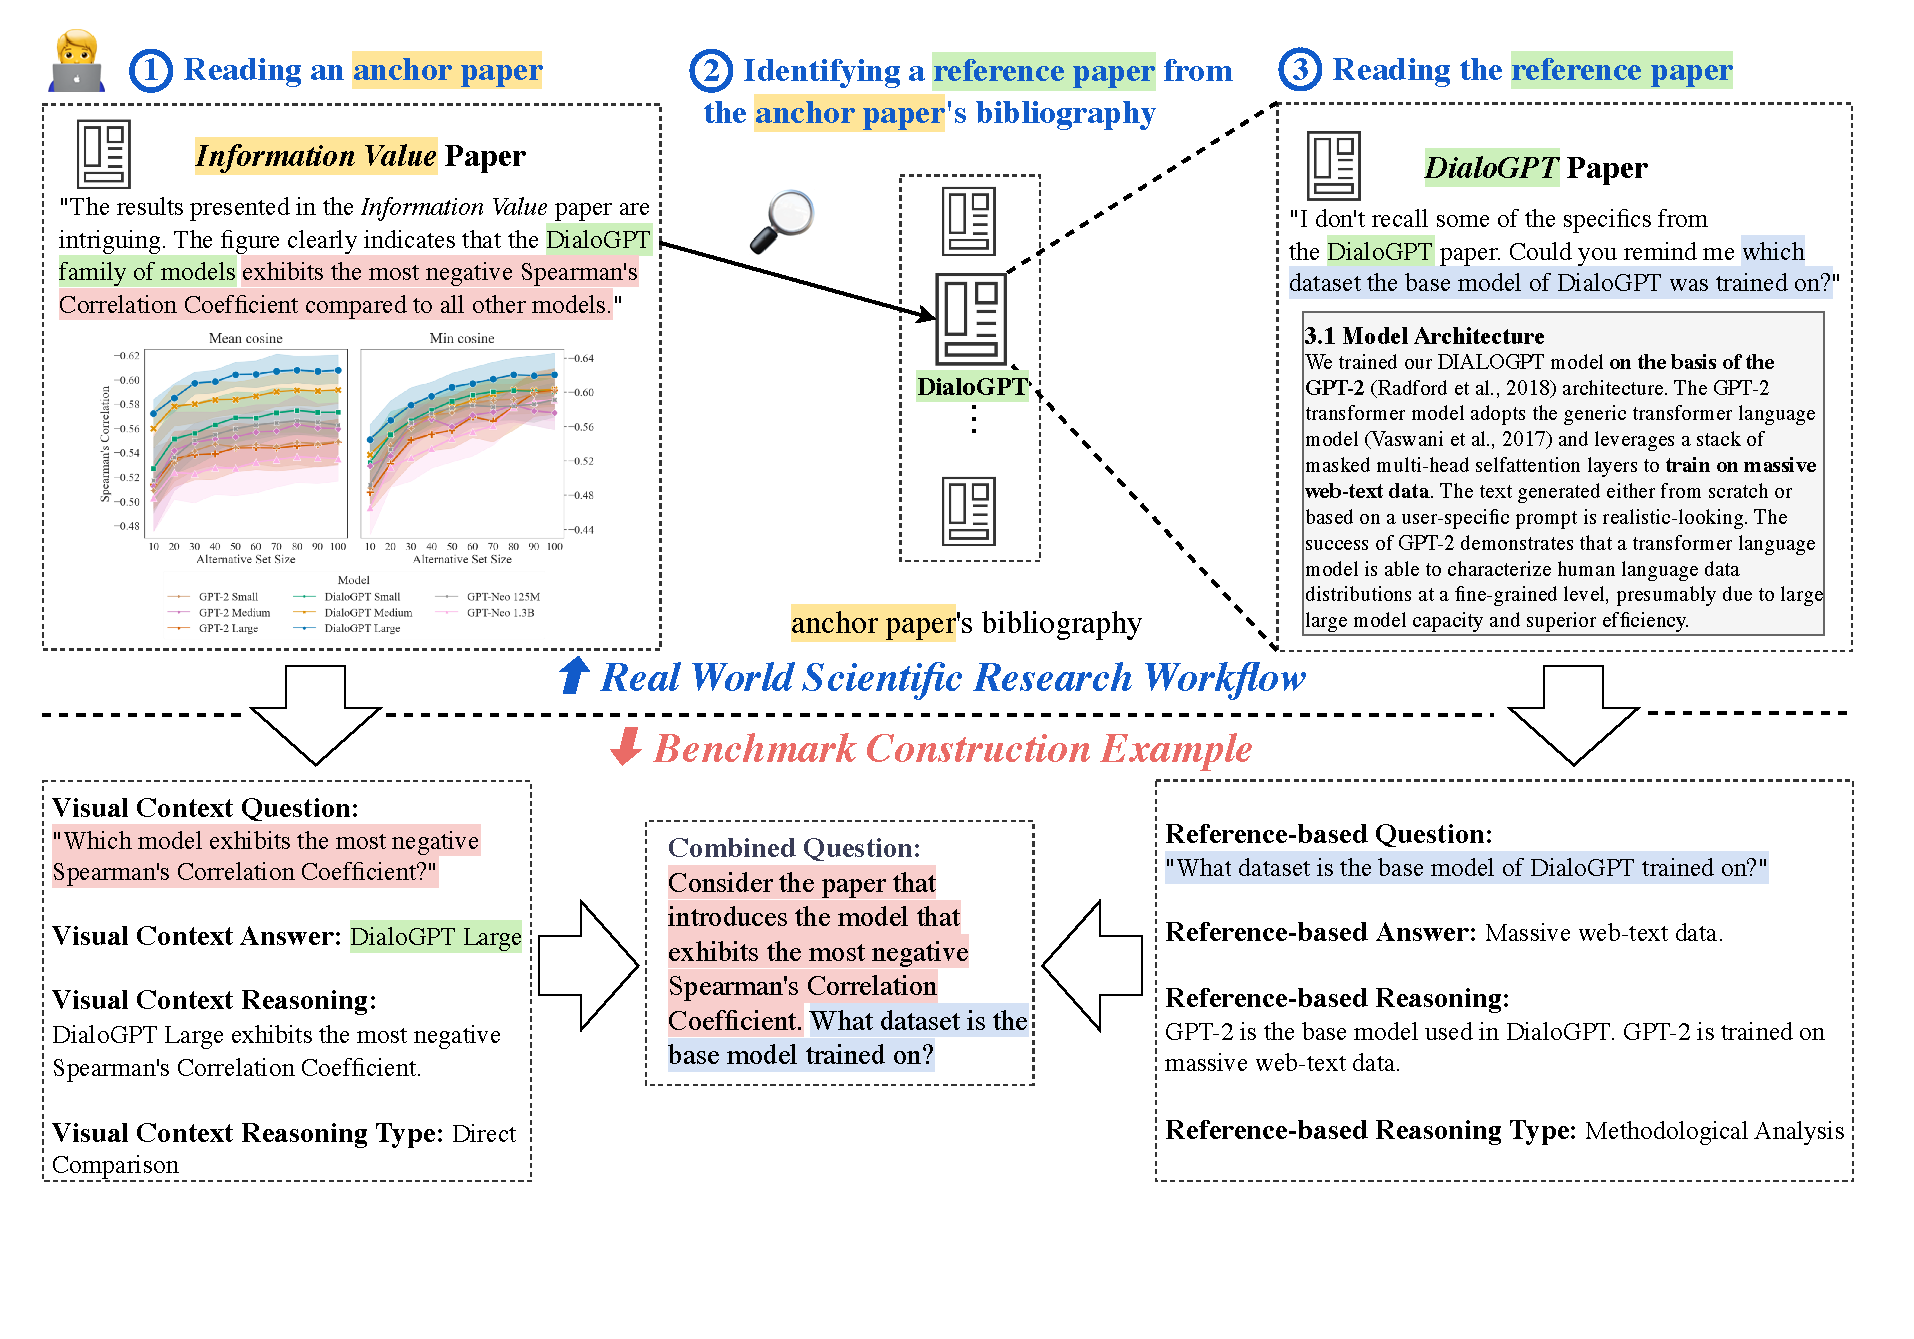
\includegraphics[width=1\textwidth]{raw_figures/figure_1.pdf}
\caption{
(\textbf{Top}) The common workflow of comparative analysis in scientific research, particularly when a result, such as a figure/table in the \hlanchor{Information Value paper (anchor paper)} \citep{giulianelli2023information}, prompts further examination of related research, such as details from \hlreference{DialoGPT (reference paper)} \citep{zhang2020dialogpt}. \textbf{(Bottom)} A demonstration of the workflow for constructing a \hllocality{visual context question}, \hldetail{reference-based question}, and combined question.
}


\label{fig:real_world}
\end{figure*}